\documentclass[tikz,border=0pt]{standalone}
% Shared visual language for every block diagram in figures/diagrams.
% Build with XeLaTeX (see figures/diagrams/build.sh).
\usepackage{fontspec}
\setmainfont{Inter}[Numbers=Lining]
\setmonofont{DejaVu Sans Mono}[Scale=0.86]
\usepackage{xcolor}
\usetikzlibrary{arrows.meta,positioning,calc,fit,backgrounds,shapes.geometric,
  shapes.misc,matrix,decorations.pathreplacing,patterns,quotes}

% Palette (matches python/figstyle.py) --------------------------------------
\definecolor{surface}{HTML}{FCFCFB}
\definecolor{ink}{HTML}{0B0B0B}
\definecolor{ink2}{HTML}{52514E}
\definecolor{muted}{HTML}{898781}
\definecolor{hair}{HTML}{E1E0D9}
\definecolor{memline}{HTML}{2A78D6}  \definecolor{memfill}{HTML}{E7F0FC}
\definecolor{aluline}{HTML}{14875E}  \definecolor{alufill}{HTML}{E3F5EE}
\definecolor{ctlline}{HTML}{B07800}  \definecolor{ctlfill}{HTML}{FDF2D9}
\definecolor{regline}{HTML}{6250D6}  \definecolor{regfill}{HTML}{ECEAFB}
\definecolor{wire}{HTML}{3D3C39}
\definecolor{accent}{HTML}{EB6834}   \definecolor{accentfill}{HTML}{FDE8DF}
\definecolor{pos}{HTML}{E34948}      \definecolor{posfill}{HTML}{FBE1E0}
\definecolor{neg}{HTML}{2A78D6}      \definecolor{negfill}{HTML}{DCE9FA}
\definecolor{zerofill}{HTML}{F0EFEC}

\tikzset{
  every picture/.style={line cap=round, line join=round, font=\small, text=ink},
  % canvas
  canvas/.style={show background rectangle,
    background rectangle/.style={fill=surface, draw=hair, rounded corners=8pt, line width=0.6pt},
    inner frame xsep=16pt, inner frame ysep=14pt},
  ttl/.style={font=\bfseries\large, anchor=north west, inner sep=0pt, text=ink},
  sub/.style={font=\small, anchor=north west, inner sep=0pt, text=ink2},
  % blocks
  blk/.style={rounded corners=3pt, line width=0.8pt, align=center, minimum height=9mm,
    inner xsep=5pt, inner ysep=3pt},
  mem/.style={blk, draw=memline, fill=memfill},
  alu/.style={blk, draw=aluline, fill=alufill},
  ctl/.style={blk, draw=ctlline, fill=ctlfill},
  reg/.style={blk, draw=regline, fill=regfill, rounded corners=1pt},
  io/.style={blk, draw=muted, fill=white},
  ghost/.style={blk, draw=muted, dashed, fill=surface},
  % arithmetic primitives
  add/.style={circle, draw=aluline, fill=white, line width=0.8pt, minimum size=6.2mm,
    inner sep=0pt, font=\normalsize},
  shf/.style={rectangle, rounded corners=1.5pt, draw=aluline, fill=white, line width=0.7pt,
    font=\ttfamily\footnotesize, inner xsep=2.5pt, inner ysep=2pt, minimum height=5mm},
  gain/.style={isosceles triangle, isosceles triangle apex angle=60, draw=aluline, fill=white,
    line width=0.7pt, inner sep=1.2pt, font=\footnotesize},
  dn/.style={circle, draw=wire, fill=white, line width=0.7pt, minimum size=8mm, inner sep=0pt,
    font=\footnotesize},
  mux/.style={trapezium, trapezium angle=72, shape border rotate=270, draw=ctlline, fill=ctlfill,
    line width=0.8pt, minimum height=13mm, minimum width=5mm, inner sep=1pt, font=\scriptsize},
  net/.style={draw=memline, fill=memfill, rounded corners=1.5pt, font=\footnotesize, inner xsep=3pt,
    inner ysep=1.6pt, minimum width=5.5mm, minimum height=4.8mm},
  % wires
  sig/.style={-{Latex[length=2.2mm,width=1.6mm]}, draw=wire, line width=0.75pt},
  bus/.style={-{Latex[length=2.6mm,width=2mm]}, draw=wire, line width=1.5pt},
  ctrl/.style={-{Latex[length=1.8mm,width=1.4mm]}, draw=ctlline, line width=0.65pt, dash pattern=on 3pt off 2pt},
  nohead/.style={-, draw=wire, line width=0.75pt},
  dot/.style={circle, fill=wire, inner sep=0pt, minimum size=3.2pt},
  % labels
  lbl/.style={font=\footnotesize, text=ink2, fill=surface, inner sep=1.2pt},
  lblc/.style={font=\footnotesize, text=ink2, inner sep=1.2pt},
  note/.style={font=\footnotesize, text=ink2, align=left, inner sep=0pt},
  head/.style={font=\bfseries\small, text=ink, inner sep=0pt},
  code/.style={font=\ttfamily\footnotesize, text=ink},
  group/.style={draw=hair, fill=white, rounded corners=6pt, line width=0.8pt, inner sep=7pt},
  grouplabel/.style={font=\bfseries\footnotesize, text=muted, anchor=south west, inner sep=2pt},
}

% Layers: groups sit above the canvas background and below the main layer.
\pgfdeclarelayer{groups}
\pgfsetlayers{background,groups,main}

% A register: box with a clock wedge at the bottom edge.
\newcommand{\clk}[1]{\draw[regline, line width=0.6pt] ($(#1.south)+(-1.4mm,0)$) -- ($(#1.south)+(0,1.6mm)$) -- ($(#1.south)+(1.4mm,0)$);}
% Bus width tick: \bw{(point)}{width}
\newcommand{\bw}[2]{\draw[wire, line width=0.6pt] ($#1+(-0.9mm,-1.2mm)$) -- ($#1+(0.9mm,1.2mm)$); \node[font=\scriptsize, text=ink2, above=0.4mm, inner sep=0.5pt] at #1 {#2};}
\newcommand{\var}[1]{\textit{#1}}
\newcommand{\usub}[1]{\ifcase#1 ₀\or ₁\or ₂\or ₃\or ₄\or ₅\fi}
\AtBeginDocument{\hyphenpenalty=10000\exhyphenpenalty=10000}

\begin{document}
\begin{tikzpicture}[canvas]
  \node[ttl] at (0,0) {One level of the separable 2-D DWT};
  \node[sub] at (0,-0.62) {Filter every row with the 1-D pair and keep every second column, then filter every column and keep every second row.};
  \def\S{4.3cm}
  % image row ------------------------------------------------------------
  \node[inner sep=0pt, anchor=north west] (i0) at (0.2,-1.65) {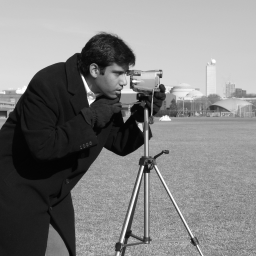
\includegraphics[width=\S]{img/input.png}};
  \node[inner sep=0pt, right=3.4cm of i0] (i1) {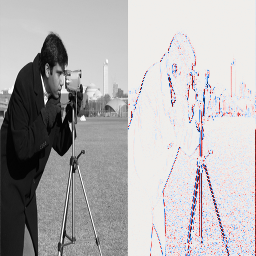
\includegraphics[width=\S]{img/rows.png}};
  \node[inner sep=0pt, right=3.4cm of i1] (i2) {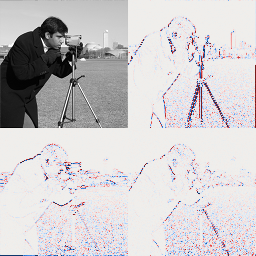
\includegraphics[width=\S]{img/packed.png}};
  \foreach \n in {i0,i1,i2} \draw[hair, line width=0.6pt] (\n.south west) rectangle (\n.north east);
  \draw[surface, line width=1.4pt] (i1.north) -- (i1.south);
  \draw[surface, line width=1.4pt] (i2.north) -- (i2.south);
  \draw[surface, line width=1.4pt] (i2.west) -- (i2.east);
  \node[head, anchor=south west] at ($(i0.north west)+(0,1.5mm)$) {Image  \var{H} × \var{W}};
  \node[head, anchor=south west] at ($(i1.north west)+(0,1.5mm)$) {After the row pass};
  \node[head, anchor=south west] at ($(i2.north west)+(0,1.5mm)$) {After the column pass};
  \tikzset{tag/.style={font=\bfseries\footnotesize, fill=surface, fill opacity=0.88, text opacity=1, inner sep=2pt, rounded corners=1.5pt, anchor=north west}}
  \node[tag] at ($(i1.north west)+(1.2mm,-1.2mm)$) {L};
  \node[tag] at ($(i1.north)+(1.2mm,-1.2mm)$) {H};
  \node[tag] at ($(i2.north west)+(1.2mm,-1.2mm)$) {LL};
  \node[tag] at ($(i2.north)+(1.2mm,-1.2mm)$) {LH};
  \node[tag] at ($(i2.west)+(1.2mm,-1.2mm)$) {HL};
  \node[tag] at ($(i2.center)+(1.2mm,-1.2mm)$) {HH};
  \draw[bus] ($(i0.east)+(2mm,0)$) -- node[note, above=2mm, align=center] {each row:\\\var{H}₀ | \var{H}₁, ↓2} node[note, below=2mm, align=center] {\var{H} × \var{W}/2 each} ($(i1.west)+(-2mm,0)$);
  \draw[bus] ($(i1.east)+(2mm,0)$) -- node[note, above=2mm, align=center] {each column:\\\var{H}₀ / \var{H}₁, ↓2} node[note, below=2mm, align=center] {\var{H}/2 × \var{W}/2 each} ($(i2.west)+(-2mm,0)$);

  % branch tree ------------------------------------------------------------
  \def\ty{-9.75}
  \node[io, minimum width=11mm] (x) at (0.75,\ty) {\var{x}};
  \node[alu, minimum width=26mm] (r0) at (4.2,\ty+1.25) {rows · \var{H}₀ · ↓2};
  \node[alu, minimum width=26mm] (r1) at (4.2,\ty-1.25) {rows · \var{H}₁ · ↓2};
  \node[mem, minimum width=9mm] (L) at (7.15,\ty+1.25) {L};
  \node[mem, minimum width=9mm] (H) at (7.15,\ty-1.25) {H};
  \node[alu, minimum width=29mm] (c00) at (10.6,\ty+1.9) {columns · \var{H}₀ · ↓2};
  \node[alu, minimum width=29mm] (c01) at (10.6,\ty+0.6) {columns · \var{H}₁ · ↓2};
  \node[alu, minimum width=29mm] (c10) at (10.6,\ty-0.6) {columns · \var{H}₀ · ↓2};
  \node[alu, minimum width=29mm] (c11) at (10.6,\ty-1.9) {columns · \var{H}₁ · ↓2};
  \foreach \s/\t/\y in {c00/LL/1.9, c01/HL/0.6, c10/LH/-0.6, c11/HH/-1.9}
    \node[mem, minimum width=11mm, minimum height=8mm] (\t) at (14.15,\ty+\y) {\t};
  \draw[sig] (x.east) -- ++(0.45,0) |- (r0.west);
  \draw[sig] (x.east) -- ++(0.45,0) |- (r1.west);
  \node[dot] at ($(x.east)+(0.45,0)$) {};
  \draw[sig] (r0) -- (L);
  \draw[sig] (r1) -- (H);
  \draw[sig] (L.east) -- ++(0.35,0) |- (c00.west);
  \draw[sig] (L.east) -- ++(0.35,0) |- (c01.west);
  \draw[sig] (H.east) -- ++(0.35,0) |- (c10.west);
  \draw[sig] (H.east) -- ++(0.35,0) |- (c11.west);
  \node[dot] at ($(L.east)+(0.35,0)$) {};
  \node[dot] at ($(H.east)+(0.35,0)$) {};
  \foreach \s/\t in {c00/LL, c01/HL, c10/LH, c11/HH} \draw[sig] (\s) -- (\t);
  \node[note, anchor=west] at ($(LL.east)+(3mm,0)$) {approximation · low-pass both ways};
  \node[note, anchor=west] at ($(HL.east)+(3mm,0)$) {horizontal edges · vertical high-pass};
  \node[note, anchor=west] at ($(LH.east)+(3mm,0)$) {vertical edges · horizontal high-pass};
  \node[note, anchor=west] at ($(HH.east)+(3mm,0)$) {diagonal detail · high-pass both ways};
  \node[grouplabel, anchor=south west] at (0.2,\ty+2.65) {THE FOUR BRANCHES · NAME = VERTICAL FILTER, THEN HORIZONTAL FILTER};
  \node[note, anchor=north west, text width=19.5cm] at (0.2,\ty-2.75) {%
    Packed layout used by every implementation: [LL LH ; HL HH], each band \var{H}/2 × \var{W}/2. The operations are linear and separable, so the column pass may run first (ARCH 5) with identical coefficients.};
\end{tikzpicture}
\end{document}
